\begin{frame}
\frametitle{Problem Statement-Quadrilateral Exercise}
\begin{enumerate}[label=(\roman*)]
\item The side AB of a parallelogram ABCD is produced to any point P. A line through A and
parallel to CP meets CB produced at Q and then parallelogram PBQR is completed. Show
that ar(ABCD) = ar(PBQR).
\textbf{Soln:}\\
Given:- CP $\parallel$ AQ
  \end{enumerate} 
\url{https://github.com/Rajolep/_Geometry/blob/master/codes/quadr/quadexer.py}
\begin{figure}
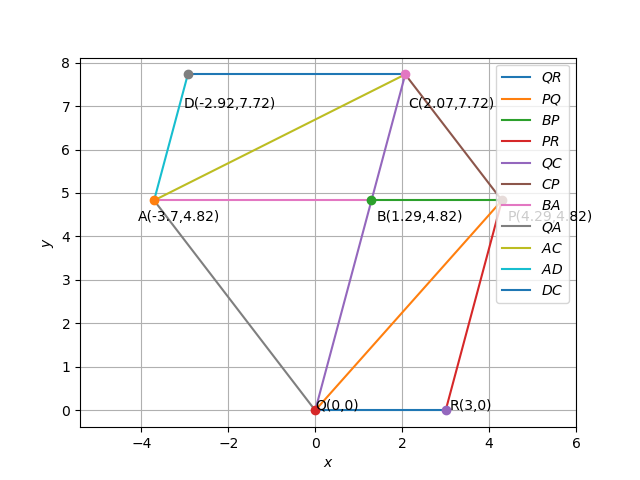
\includegraphics[scale=0.3]{./figs/quadexer.png}
\end{figure}
\end{frame}
\begin{frame}
\begin{figure}
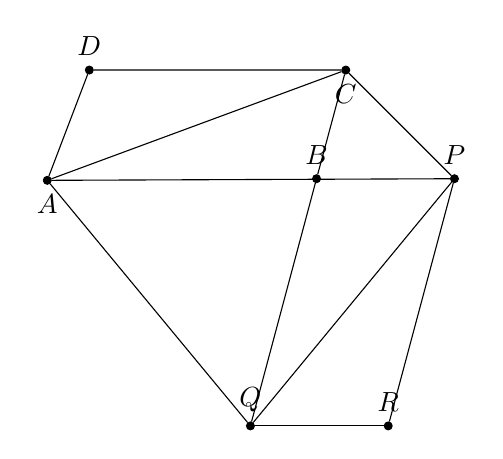
\begin{tikzpicture}
[scale =0.5,>=stealth,point/.style = {draw, circle, fill = black, inner sep = 1pt},]
\node (D) at (-4.0921,9.0388)[point,label=above :$D$] {};
\node (C) at (2.42196,9.03888)[point,label=below :$C$] {};
\node (A) at (-5.16,6.2375)[point,label=below :$A$] {};
\node (B) at (1.67905,6.2787)[point,label=above :$B$] {};
\node (P) at (5.18232,6.278517)[point,label=above :$P$] {};
\node (Q) at (0,0)[point,label=above :$Q$] {};
\node (R) at (3.5,0)[point,label=above :$R$] {};
\draw (A)--(P);
\draw (C)--(P);
\draw (B)--(C);
\draw (C)--(D);
\draw (D)--(A);
\draw (P)--(R);
\draw (C)--(A);
\draw (P)--(Q);
\draw (B)--(Q);
\draw (R)--(Q);
\draw (A)--(Q);
\end{tikzpicture}

\end{figure}
\url{https://github.com/Rajolep/_Geometry/blob/master/figs/quadexe.tex}
\end{frame}
\begin{frame}
\begin{itemize}
\item Q=$\myvec{0\\0}$    R=$\myvec{3\\0}$   $\angle{QRP}=\degree(105)$\\
\item QP=$\sqrt{a^2+b^2-2ab\cos{105}}$
\item P=$\myvec{p\\q}$  a=3, b=5 c=QP\\
\item p=$\frac{a^2+c^2-b^2}{2a}$    q=$\sqrt{c^2-p^2}$\\
\item P(4.29,4.82)
\item C=$\myvec{p1\\q1}$  f=b+a\\
\item CP=g=$\sqrt{f^2+c^2-2fc\cos{75}}$
\item p1=$\frac{c^2+f^2-g^2}{2c}$    q1=$\sqrt{f^2-p1^2}$\\
\item C(2.07,7.72)
\end{itemize}
\end{frame}
\begin{frame}
\begin{align*}
CP \parallel AQ\\
\end{align*}
\begin{itemize}
\item area of $\triangle{ACQ}$ =  area of $\triangle{AQP}$\\

\item subtract area$\triangle{ABQ}$ in above Eqn\\

\item ar$\triangle{ACQ}$-ar$\triangle{ABQ}$ = ar$\triangle{APQ}$-ar$\triangle{ACQ}$\\

\item ar$\triangle{ABC}$ = ar$\triangle{PBQ}$....(1)\\

\item $\triangle{ABC} \cong \triangle{ADC}$\\

\item ar$\triangle{ABC}$ = ar$\triangle{ADC}$\\

\item ar$\triangle{ABC}$ = ar$\triangle{ADC}$ = $\frac{1}{2}(ABCD)$...(2)\\
\end{itemize}
\end{frame}
\begin{frame}
similarly in PBQR,\\
$\triangle{PBQ} \cong \triangle{PRQ}$\\
ar$\triangle{PBQ}$ = ar$\triangle{PRQ}$\\
ar$\triangle{PBQ}$ = ar$\triangle{PRQ}$ = $\frac{1}{2}(ABCD)$....(3)\\
frm (1)\\
$\triangle{ABC}$ = $\triangle{PBQ}$\\
frm (2)  (3)\\
$\frac{1}{2}(ABCD)$ = $\frac{1}{2}(ABCD)$\\
Ar(ABCD) = Ar(PBQR)\\
\end{frame}